

\documentclass[11pt]{report}
\pagestyle{plain}
\usepackage[spanish]{babel}
\selectlanguage{spanish}
\usepackage[utf8]{inputenc}
\usepackage{listings}
\usepackage{color}
\usepackage[table]{xcolor}
\usepackage{graphicx}
\usepackage{amssymb}
\usepackage{url}

% ------------------- Titulo y  Autor -----------------------------
% Este documento fue creado por Alejandro Fernandez (alejandro.fernandez@lifia.info.unlp.edu.ar) en su primera version.
%Algunos cambios en 
\title{Este es el título de la tesis}
\author{Estos son los alumnos que la desarrollaron}

\begin{document}

\maketitle

\begin{abstract}
Este es un resumen de la tesis muy corto (media carilla). El que lo lee se tiene que quedar con la idea de: 1) en que tema trabajaron, 2) cual es el problema que intentaron resolver, 3) que técnica aplicaron para resolverlo y por qué es novedosa, 4) que descubrieron en el proceso (un adelanto de conclusión). 
\end{abstract}

\tableofcontents

%Cada capitulo será un archivo .tex el cual estará en su propia carpeta, con sus propias imágenes).
%El comando include hace que el capitulo respectivo se incluya en el documento. No es necesario indicar la extensión 
%del archivo dado que asume que es .tex
%Los números en el nombre de las carpetas son solo para tenerlas ordenadas.

\chapter{Introducción}
\label{introduccion}

La introducción responde cinco preguntas:
\begin{description}
\item[¿en que tema están trabajando? ] Introduce en contexto en el que están trabajando (p.e., el ámbito en el que se dá el problema). Da definiciones (brevemente) de conceptos que aparecen en el contexto. 
\item[¿cual es el problema? ¿es interesante? ] Presenta el problema que se quiso resolver (o la necesidad que se quiso cubrir), y explica por que es relevante y no es trivial resolverlo.  Introduce definiciones (brevemente) que ayuden a entender el problema. Esta parte (en conjunto con la anterior) dan la motivación del trabajo. 
\item[¿cual es la estrategia general de solución? ] Presenta en términos generales la estrategia de solución (p.e., cuenta que se desarrolló un sistema que permite... y que por su característica... resuelve el problema planteado.
\item[¿cuales son las contribuciones del trabajo? ] Enumera que es lo que obtiene quien lee el trabajo. Ejemplos de contribuciones son: un análisis detallado del problema X en el contexto Y, una comparación de tecnologías de servidores ZZZ, una revisión de literatura del estado actual del tema J, una arquitectura y diseño de un sistema que permite..., un prototipo que muestra como la arquitectura Z puede implementarse de forma B, evidencia experimental que muestra que es posible WW, un framework/libreria web para GGG, un algoritmo eficiente para ...   
\item[¿Cómo esta organizado el trabajo?] El ultimo párrafo de la Introducción explica como esta organizado el documento; como se lee, que es lo que se va a encontrar en cada capítulo y como se relacionan.   
\end{description}

Dependiendo de lo larga que quede puede tener varias secciones. No estaría mal que esas secciones se llamen ``Motivación''\footnote{prestá atención a como se ponen las comillas en LaTex} (que habla del contexto y el problema), ``Enfoque'' (que explica como lo van a hacer), ``Contribuciones'' y ``Organización''.  

Muchos dicen que la intro se puede escribir al final. De hecho, las contribuciones y la organización es algo que está claro solo al terminar el proyecto de tesis. Sin embargo, creo que tener un borrador corto de la intro (un párrafo respondiendo a cada una de las preguntas) es bueno para utilizarlo como referencia cada vez que nos olvidamos que es lo que queríamos hacer. 


\section{Algunas palabras sobre este documento}

Mi idea al escribir este documento es que sirva como punto de partida para organizar la tesis (el proyecto y el documento) y como punto de partida para editar el documento en LaTex. Hay muchas referencias en la web con guías similares. Todas tienen algo bueno. La página web de Willilam Shoaff Shoaff \cite{Shoaff} habla sobre como organizar una tesis de maestría (lo cual creo que es aplicable a la tesis de Licenciatura). Si se imaginan un futuro escribiendo artículos técnicos y están con tiempo para leer, les recomiendo el libro de Justin Zobel "Writing for Computers Science" \cite{Zobel04a} que está en biblioteca de Informática de UNLP. En la Figura \ref{zobel-page-46} se pude ver un extracto de libro en el que discute el poco valor que tienen palabras como "muy" en la escritura técnica. 

\begin{figure}
\begin{center}
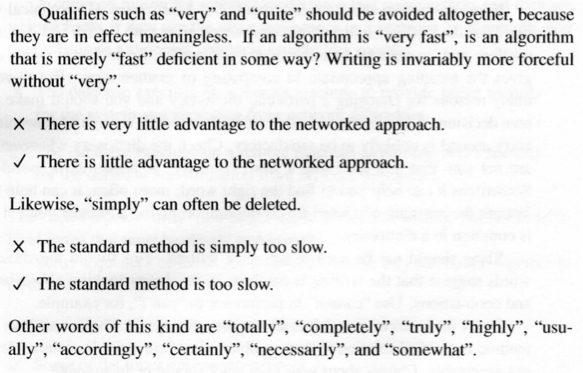
\includegraphics[width=0.8\textwidth]{00-introduccion/zobel-page-46}
\caption{Extracto del libro Writing for Computers Science de Justin Zobel}
\label{zobel-page-46}
\end{center}
\end{figure}


\chapter{Trabajo Relacionado}
Hacer una tesis implica encontrar una pregunta que valga la pena responder o un problema que valga la pena resolver y darle respuesta o solución. Es una tarea de investigación que tiene como aspecto muy importante conocer lo que ya existe alrededor de la pregunta o problema que se elige. 

Al llegar a este capitulo, el lector tiene una idea de cual es el problema. Seguramente se imagina problemas similares o soluciones al problema. El objetivo, en este momento, es convencerlo de que conocemos el problema y otros similares; que conocemos las formas en las que se lo ha intentado resolver (o a problemas similares); y que aún después de saber todo eso sigue siendo un problema importante, difícil y que nadie resolvió 8o nadie revolvió tan bien como nosotros).

Para escribir este capitulo hay que leer. Hay que buscar soluciones a problemas similares y compararlas con lo que nosotros queremos hacer. Si sabemos que la nuestra es mejor, ya podemos marcar cuales son los puntos débiles de las existentes. También se puede escribir un poco sobre otras investigaciones, que si bien no atacaron problemas parecidos, pueden ser aplicadas a resolver parte de este. 

Este capitulo es bueno ir escribiendolo en borrador cada vez que se lee algo (un articulo por ejemplo). Por lo menos hay que escribir un resumen de un párrafo de lo leído (registrando la referencia en el archivo bibliografia.bib y citando dede acá), y dar nuestra opinión al respecto en términos de su relación con el problema de nuestra tesis.

%Sección agregada por Diego Torres. Mayo 2019.
\section{Fuentes de Información}

Esta sección es una de las que demuestra más complejidad de escribir, al menos en la experiencia que tuve en la dirección de tesinas de grado en la Facultad de Informática de la UNLP, ya que la misma implica leer sobre trabajos relacionados y poder explicarlos dentro del contexto de vuestro trabajo. 

Leer implica también buscar dónde leer. A veces no es sencillo si no posees entrenamiento. Algo en lo que prestar mucha atención es en las fuentes de información. 

Particularmente prefiero las siguientes fuentes de información, porque considero que le dan mayor sustento a lo que justifiquemos e intentemos aportar al campo científico:
\begin{itemize}
    \item Artículos científicos de revistas (journals) o de conferencias. Ambos actualizados y en lo posible citados por otros trabajos. Esto último puede ser relativo al tiempo en que fueron publicados. 
    \item Libros. Referentes en la disciplina.
\end{itemize}

Por otro lado, trato de no incluir
\begin{itemize}
    \item Páginas web.
    \item Documentos sueltos que se encuentran por internet. Por ejemplo, artículos de divulgación.
\end{itemize}

Para poder encontrar artículos científicos, una herramienta muy útil es Google Scholar \footnote{\url{http://scholar.google.com}}. Es una versión del famoso buscador destinado a basar sus búsquedas en artículos científicos. 


\section{Citar y no copiar}

A medida que vamos leyendo sobre otros trabajos relacionados o sobre articulo que describen parte del contexto que le da forma al problema que resolvemos en esta tesis, nos vamos a dar cuenta que existen otras miradas y acercamientos a un mismo problema. Muchas veces, nos va a parecer que no existe otra forma mejor de explicar lo mismo si no es con las palabras que le dieron los autores de los artículos que leímos. 

Sin embargo, la tesina de grado es un espacio donde los autores (alumnos que van a recibirse de licenciados) deben producir el contenido de la misma. 

Las fuentes bibliográficas que leemos nos van a servir para diferentes cosas. Principalmente para darle sustento a algo que afirmamos, por ejemplo:

``sabemos que es posible algoritmicamente encontrar el camino de distancia mínima entre dos nodos pertenecientes a un grafo \cite{dijkstra1959note}''

La afirmación desde ``sabemos'' hasta ``grafo'' es una producción de quien escribió la frase, sin embargo esto esta fundado en el artículo escrito posiblemente por otra persona en la cita que se encuentra codificada luego, en este caso con \cite{dijkstra1959note} y que se listará al final en la sección de bibliografía.
\chapter{Estrategia general}
\label{estrategia}

Un tipo de tesis común en Sistemas es la que propone una solución a un problema \footnote{hay otros tipos, por ejemplo aquellas que demuestran experimentalmente alguna cualidad de algún fenómeno}. Puede ser que el problema todavía no haya sido resuelto (poco probable); o puede ser que se proponga una solución que es mejor a las existentes en algún aspecto. Una forma interesante de imaginar el documento de tesis es como un espiral, que da cuatro vueltas, de adentro para afuera. En cada vuelta da mas detalles.

\begin{itemize}
\item Vuelta 1 (el resumen): se cuenta toda la tesis (problema, estrategia de solución, resultado obtenido) en un solo párrafo.
\item Vuelta 2 (la introducción): En la introducción, se vuelve a contar el problema (ahora se introduce el contexto, se explica por que es un problema relevante y difícil, se dan algunas definiciones), se adelanta cual es la estrategia de solución aunque todavía no se puede explicar mucho, se listan las contribuciones principales.  
\item Vuelta 3 (varios capítulos): Ahora se puede dedicar un capitulo completo a contar bien cual es la estrategia general (que método se aplica, que arquitectura, que tecnologías, que pasos tiene la solución, etc), y se puede dedicar un capitulo completo a cada parte interesante de la solución (esto depende mucho de lo que resuelvas y que partes imprtantes tenga).
\end{itemize}  

El capitulo de estrategia general tiene como objetivo contar cual es la estrategia/método de solución al problema elegido.  Por ejemplo, ¿se propone una metodología? ¿que pasos tiene? ¿Se construye un sistema? ¿que arquitectura tiene? ¿que partes importantes tiene? ¿que funcionalidad provee?

Con este capítulo le debería alcanzar al que lee para entender como se resolvió el problema. Los capítulos que siguen a este pueden dar mas detalle sobre aquellos aspectos/partes que valga la pena detallar.  De alguna forma, este capitulo es el mapa que ordena los capítulos que siguen. 







\chapter{Capítulo específico}

Al capitulo \ref{estrategia}, que describe la estrategia general, lo siguen varios capítulos que entran en detalle en distintas partes de la solución. Uno, por ejemplo, puede describir el modelo de datos que utiliza la aplicación, otro puede describir el front-end de la aplicación, otro puede describir el algoritmo de recomendación de nuevos contenidos, etc. Por lo general hay que explicar en detalle aquellas cosas que no son obvias para quien no hizo la tesis y que las necesitaría si quiere reproducir lo que ustedes hicieron. 

No es necesario escribir mucho. Simplemente es cuestión de preguntarse que le podría resultar interesante o novedoso a
un compañero de estudio que no conoce el tema. 



\chapter{Evaluación}

Supongamos que se quiso atacar el problema de la dificultad en el desarrollo de aplicaciones móviles multi-plataforma. Y que lo que se hizo fue desarrollar una librería de clases. ¿Cómo demuestro que la librería de clases resuelve el problema?

Antes que nada, deberíamos haber dejado claro, en alguna sección del capítulo \ref{introduccion} cuales son los indicadores que miro para decir que hay "dificultad en el desarrollo de aplicaciones móviles". Por ejemplo, ¿cantidad de bugs específicos de la plataforma? ¿tiempo que lleva traducir los aspectos específicos?. Conocer esos indicadores (o aspectos) es importante para decidir a cuales de ellos voy a apuntar en mi solución (porque tal vez no puedo ser mejor en todos los aspectos). Es importante para poder comparar mi solución con otras. Y es importante porque en este capítulo tengo que demostrar que mi solución es mejor en términos del/los aspectos elegidos. 

La evaluación se puede hacer de muchas formas y depende del caso en particular. Por ejemplo, podrías poner a varios compañeros a hacer la misma aplicación demo con tu librería y otras que ellos quieran. Y luego les hacés preguntas para saber si con tu libreria fué mejor. O podés contar la cantidad de bugs que se hicieron usando tu librería vs los que se hicieron sin ella. Hacer un experimento es complejo, pero hay muchas alternativas intermedias para que puedas demostrar que tu propuesta resuelve el problema planteado.







\chapter{Conclusiones y trabajo futuro}

En el apartado de conclusiones se hace un breve resumen de lo que uno quiso hacer y lo que pudo hacer. Se sacan conclusiones respecto a la efectividad de la estrategia aplicada en resolver el problema. Se sacan conclusiones sobre la complejidad del problema y su importancia. Hasta se puede hablar de alternativas que probamos y no funcionaron. 
Esta sección es nuestra oportunidad para recordarle al lector que era un problema difícil y que pudimos resolverlo. Y de paso le recordamos la lista de contribuciones.  

Antes de terminar, hay que dejar algunas líneas para quien quiera continuar investigando el tema (trabajo futuro). ¿Qué hubiese sido bueno hacer y no se hizo porque no hubo tiempo? ¿Qué no funciona del todo bien y se podría mejorar? ¿Qué otras alternativas de solución se te ocurren ahora que podrían ser mejores? 






%Los artículos que se citan en la tesis, se incluyen en el archivo bibliografía.bib, en formato bibtex.
%En la sección bibliografía, van a aparecer automáticamente aquellos que se citan desde el texto 
%utilizando el comando \cite con la etiqueta correspondiente - en la introducción hay un par de ejemplos. 

\bibliographystyle{ieeetr}
\bibliography{90-bibliografia}


\end{document}
\end

